\documentclass{beamer}% This is the file main.tex
\usepackage{graphicx}
\usepackage{outlines}
\usepackage{gensymb}
\usepackage{pgfplots}
\pgfplotsset{compat=1.11}
\usepackage{tikz}


\usetheme{Boadilla}
\title{Choosing Gear Ratios}
\author{Thad Hughes}
\date{\today}

\hypersetup{%
  colorlinks=false,% hyperlinks will be black
  linkbordercolor=red,% hyperlink borders will be red
  pdfborderstyle={/S/U/W 1}% border style will be underline of width 1pt
}

\begin{document}

\maketitle

\begin{frame}
\frametitle{Outline}
\framesubtitle{Where are we going today?}

\begin{outline}
	\1 Goals
	\1 The general DE and Behavior
\end{outline}

\begin{block}{}
	This may or may not be review for you. If it is, skim through, make sure you're comfy. If not, let this be a fun first foray!
\end{block}

\end{frame}

\begin{frame}
	\frametitle{Goals of a Mechanism}
	\begin{itemize}
		\item Move/lift a load to a position
		\item Move/lift a load to a velocity
		\item Minimize electrical consumption
		\item Maximize precision/controllability
	\end{itemize}
\end{frame}

\begin{frame}
	\frametitle{What is motor behavior like? (Flywheel Example)}
	\framesubtitle{Building on Motor Behavior}

	\begin{equation}
		T_{motor} = T_{max} \frac{(\omega_{max}-\omega)}{\omega_{max}}
	\end{equation}	
	
	\begin{equation}
		T_{gearbox} = G T_{motor}
	\end{equation}
	
	A flywheel with torques acting on it can be modeled as:
	
	\begin{columns}
	\column{0.5\textwidth}
	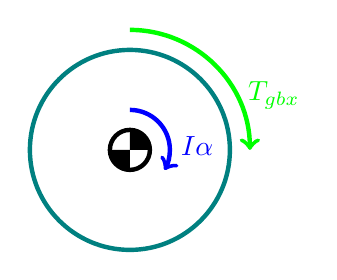
\begin{tikzpicture}[x=1.0in,y=1.0in]
		\draw[ultra thick] (0,0) circle (0.1);
		\fill[black] (0,0.1)--(0,0)--(0.1,0) arc[start angle=0, end angle=90, radius=0.1]--cycle;
		\fill[black] (0,-0.1)--(0,0)--(-0.1,0) arc[start angle=180, end angle=270, radius=0.1]--cycle;
		\draw[ultra thick, teal] (0,0) circle (0.5);
		
		%\draw[ultra thick, red, ->] (0,0.6) arc[start angle=90, end angle=180, radius=0.6] node[pos=0.7,left]{$M_{resist}$};
		\draw[ultra thick, green, ->] (0,0.6) arc[start angle=90, end angle=0, radius=0.6] node[pos=0.7,right]{$T_{gbx}$};
		
		\draw[ultra thick, blue, ->] (0,0.2) arc[start angle=90, end angle=-30, radius=0.2] node[pos=0.7,right]{$I \alpha$};
	\end{tikzpicture}	
	\column{0.5\textwidth}
	\begin{equation}
		\sum M = I \alpha
	\end{equation} 
	\begin{equation}
		T_{gbx} = I \alpha_{wheel}
	\end{equation}
	
	\end{columns}
	
\end{frame}

\begin{frame}
	\frametitle{What is motor behavior like? (Continued)}
%	\framesubtitle{Building on Motor Behavior}
	\begin{equation}
		\alpha_{wheel} = \frac{d \omega_{wheel}}{dt}
	\end{equation}\begin{equation}
		\omega_{motor} = G \omega_{wheel}
	\end{equation}\begin{equation}
		G T_{max} \frac{\omega_{max} - \omega}{\omega_{max}} = \frac{I}{G} \frac{d \omega}{dt}
	\end{equation}
	
		This is a "differential equation" ($\frac{d \omega}{dt}$ and $\omega$ are in the same equation).	
	
	\begin{alertblock}{Apology}
		This math isn't too imperative to the overall point. If you prefer to just use the calculator and look at pretty plots and trends, that's alright.
		
		There be dragons (calculus) ahead.
	\end{alertblock}	
	
\end{frame}

\begin{frame}
	\frametitle{The Mathy Approach}
	
	We can solve differential equations with math!	
	\begin{equation}
		\mbox{let } B = \frac{G^2 T_{max}}{I}
	\end{equation}\begin{equation}
		\mbox{Substitute: } B\ \frac{\omega_{max} - \omega}{\omega_{max}} = \frac{d \omega}{d t}
	\end{equation}\begin{equation}
		\mbox{Separate and integrate: } \int B\ dt = \int \frac{\omega_{max}}{\omega_{max} - \omega} d \omega
	\end{equation}\begin{equation}
		\mbox{Solve integral: } B t + C = -\omega_{max}\ ln[\omega_{max} - \omega]
	\end{equation}\begin{equation}
		\mbox{Solve for $\omega$: } \omega = \omega_{max} - C\ e^{-\frac{B t}{\omega{max}}}
	\end{equation}\begin{equation}
		\mbox{Solve for C with initial condition } \omega(0) = 0 \rightarrow C = \omega_{max}
	\end{equation}\begin{equation}
		\omega = \omega_{max}\ [1 - e^{-\frac{G^2\ T_{max}\ t}{I\ \omega{max}}}]
	\end{equation}\begin{equation}
		\omega_{gbx} = \frac{\omega_{max}}{G}\ [1 - e^{-\frac{G^2\ T_{max}\ t}{I\ \omega{max}}}]
	\end{equation}
\end{frame}

\begin{frame}
	\frametitle{Plotting the Math}
	\begin{columns}
	\column{0.35\textwidth}
		\begin{block}{}
			Acceleration is the slope of the velocity curve.
		\end{block}
		
		\begin{block}{}
		Increasing the mass of the system (or decreasing power!) will decrease acceleration.
		\end{block}\begin{block}{}		
		Increasing the gear ratio of the system will increase acceleration, but decrease maximum speed.
		\end{block}
		
	\column{0.62\textwidth}
	\centering
	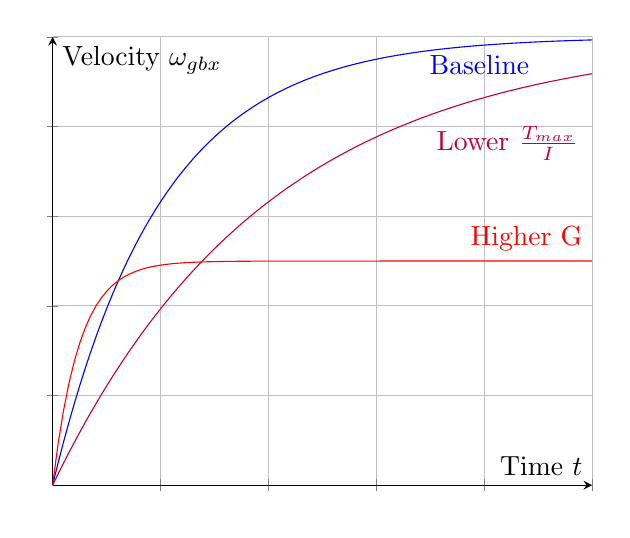
\begin{tikzpicture}[x=1.0in,y=1.0in]
		%\draw[gray] (0,0)--(3,0) node[pos=0.5,below,black]{Time $t$};
		%\draw[gray] (0,0)--(0,2) node[pos=0.5,above,rotate=90,black]{Ang. Velocity $\omega_{gbx}$};
		
		%\draw[red] (0,0)
		
		\begin{axis}[grid=both,
          xmax=5,ymax=1,
          xticklabel=\empty, yticklabel=\empty,
          axis lines=middle,
          restrict y to domain=-7:12,
          xlabel={Time $t$},
          ylabel={Velocity $\omega_{gbx}$}
          ]
		\addplot[blue,domain=0:5,samples=100]  {1*(1-exp(-1^2*x))} node[pos=0.8,below] {Baseline};
		\addplot[purple,domain=0:5,samples=100]  {1*(1-exp(-1^2/2*x))} node[pos=0.7,below right] {Lower $\frac{T_{max}}{I}$};
		\addplot[red,domain=0:5,samples=100]  {1/2*(1-exp(-2^2*x))} node[above left] {Higher G};
		\end{axis}
	\end{tikzpicture}
	\begin{alertblock}{Warning}
			This assumes that there is no constant load, or friction.
			This behavior is generally true, but not exactly true.
		\end{alertblock}
	\end{columns}
\end{frame}

\begin{frame}
	\frametitle{Simulating (Actually... is easier!)}
\end{frame}

\end{document}